% Options for packages loaded elsewhere
% Options for packages loaded elsewhere
\PassOptionsToPackage{unicode}{hyperref}
\PassOptionsToPackage{hyphens}{url}
\PassOptionsToPackage{dvipsnames,svgnames,x11names}{xcolor}
%
\documentclass[
  11pt,
  letterpaper,
  DIV=11,
  numbers=noendperiod]{scrartcl}
\usepackage{xcolor}
\usepackage[margin=1in]{geometry}
\usepackage{amsmath,amssymb}
\setcounter{secnumdepth}{2}
\usepackage{iftex}
\ifPDFTeX
  \usepackage[T1]{fontenc}
  \usepackage[utf8]{inputenc}
  \usepackage{textcomp} % provide euro and other symbols
\else % if luatex or xetex
  \usepackage{unicode-math} % this also loads fontspec
  \defaultfontfeatures{Scale=MatchLowercase}
  \defaultfontfeatures[\rmfamily]{Ligatures=TeX,Scale=1}
\fi
\usepackage{lmodern}
\ifPDFTeX\else
  % xetex/luatex font selection
  \setmainfont[]{Times New Roman}
\fi
% Use upquote if available, for straight quotes in verbatim environments
\IfFileExists{upquote.sty}{\usepackage{upquote}}{}
\IfFileExists{microtype.sty}{% use microtype if available
  \usepackage[]{microtype}
  \UseMicrotypeSet[protrusion]{basicmath} % disable protrusion for tt fonts
}{}
\makeatletter
\@ifundefined{KOMAClassName}{% if non-KOMA class
  \IfFileExists{parskip.sty}{%
    \usepackage{parskip}
  }{% else
    \setlength{\parindent}{0pt}
    \setlength{\parskip}{6pt plus 2pt minus 1pt}}
}{% if KOMA class
  \KOMAoptions{parskip=half}}
\makeatother
% Make \paragraph and \subparagraph free-standing
\makeatletter
\ifx\paragraph\undefined\else
  \let\oldparagraph\paragraph
  \renewcommand{\paragraph}{
    \@ifstar
      \xxxParagraphStar
      \xxxParagraphNoStar
  }
  \newcommand{\xxxParagraphStar}[1]{\oldparagraph*{#1}\mbox{}}
  \newcommand{\xxxParagraphNoStar}[1]{\oldparagraph{#1}\mbox{}}
\fi
\ifx\subparagraph\undefined\else
  \let\oldsubparagraph\subparagraph
  \renewcommand{\subparagraph}{
    \@ifstar
      \xxxSubParagraphStar
      \xxxSubParagraphNoStar
  }
  \newcommand{\xxxSubParagraphStar}[1]{\oldsubparagraph*{#1}\mbox{}}
  \newcommand{\xxxSubParagraphNoStar}[1]{\oldsubparagraph{#1}\mbox{}}
\fi
\makeatother


\usepackage{longtable,booktabs,array}
\usepackage{calc} % for calculating minipage widths
% Correct order of tables after \paragraph or \subparagraph
\usepackage{etoolbox}
\makeatletter
\patchcmd\longtable{\par}{\if@noskipsec\mbox{}\fi\par}{}{}
\makeatother
% Allow footnotes in longtable head/foot
\IfFileExists{footnotehyper.sty}{\usepackage{footnotehyper}}{\usepackage{footnote}}
\makesavenoteenv{longtable}
\usepackage{graphicx}
\makeatletter
\newsavebox\pandoc@box
\newcommand*\pandocbounded[1]{% scales image to fit in text height/width
  \sbox\pandoc@box{#1}%
  \Gscale@div\@tempa{\textheight}{\dimexpr\ht\pandoc@box+\dp\pandoc@box\relax}%
  \Gscale@div\@tempb{\linewidth}{\wd\pandoc@box}%
  \ifdim\@tempb\p@<\@tempa\p@\let\@tempa\@tempb\fi% select the smaller of both
  \ifdim\@tempa\p@<\p@\scalebox{\@tempa}{\usebox\pandoc@box}%
  \else\usebox{\pandoc@box}%
  \fi%
}
% Set default figure placement to htbp
\def\fps@figure{htbp}
\makeatother

\ifLuaTeX
  \usepackage{luacolor}
  \usepackage[soul]{lua-ul}
\else
  \usepackage{soul}
\fi




\setlength{\emergencystretch}{3em} % prevent overfull lines

\providecommand{\tightlist}{%
  \setlength{\itemsep}{0pt}\setlength{\parskip}{0pt}}



 


\usepackage{booktabs}
\usepackage{caption}
\usepackage{longtable}
\usepackage{colortbl}
\usepackage{array}
\usepackage{anyfontsize}
\usepackage{multirow}
\KOMAoption{captions}{tableheading}
\numberwithin{figure}{section}
\makeatletter
\@ifpackageloaded{caption}{}{\usepackage{caption}}
\AtBeginDocument{%
\ifdefined\contentsname
  \renewcommand*\contentsname{Table of contents}
\else
  \newcommand\contentsname{Table of contents}
\fi
\ifdefined\listfigurename
  \renewcommand*\listfigurename{List of Figures}
\else
  \newcommand\listfigurename{List of Figures}
\fi
\ifdefined\listtablename
  \renewcommand*\listtablename{List of Tables}
\else
  \newcommand\listtablename{List of Tables}
\fi
\ifdefined\figurename
  \renewcommand*\figurename{Figure}
\else
  \newcommand\figurename{Figure}
\fi
\ifdefined\tablename
  \renewcommand*\tablename{Table}
\else
  \newcommand\tablename{Table}
\fi
}
\@ifpackageloaded{float}{}{\usepackage{float}}
\floatstyle{ruled}
\@ifundefined{c@chapter}{\newfloat{codelisting}{h}{lop}}{\newfloat{codelisting}{h}{lop}[chapter]}
\floatname{codelisting}{Listing}
\newcommand*\listoflistings{\listof{codelisting}{List of Listings}}
\makeatother
\makeatletter
\makeatother
\makeatletter
\@ifpackageloaded{caption}{}{\usepackage{caption}}
\@ifpackageloaded{subcaption}{}{\usepackage{subcaption}}
\makeatother
\usepackage{bookmark}
\IfFileExists{xurl.sty}{\usepackage{xurl}}{} % add URL line breaks if available
\urlstyle{same}
\hypersetup{
  pdftitle={Bridging the Gap:},
  pdfauthor={Brock Akerman, Hanan Ali, Taylor Cesarski},
  colorlinks=true,
  linkcolor={blue},
  filecolor={Maroon},
  citecolor={Blue},
  urlcolor={Blue},
  pdfcreator={LaTeX via pandoc}}


\title{Bridging the Gap:}
\usepackage{etoolbox}
\makeatletter
\providecommand{\subtitle}[1]{% add subtitle to \maketitle
  \apptocmd{\@title}{\par {\large #1 \par}}{}{}
}
\makeatother
\subtitle{Comparing Employer and Educator Expectations in Small Animal
Dentistry}
\author{Brock Akerman, Hanan Ali, Taylor Cesarski}
\date{2025-06-25}
\begin{document}
\maketitle

\renewcommand*\contentsname{Table of contents}
{
\hypersetup{linkcolor=}
\setcounter{tocdepth}{2}
\tableofcontents
}

\section{Abstract}\label{abstract}

Authors of each section

Introduction - Taylor Cesarski Data - Brock Akerman Methods - Taylor
Cesarski Results - All

\begin{itemize}
\tightlist
\item
  Questions 1-4 - Hanan Ali
\item
  Questions 5,7 - Taylor Cesarski
\item
  Questions 6,8 - Brock Akerman
\end{itemize}

\section{Introduction}\label{introduction}

Dr.~Mariea Ross-Estrada, a faculty member at North Carolina State
University's College of Veterinary Medicine, is exploring whether there
are differences between the expectations of small animal primary care
veterinary employers and veterinary educators regarding new graduates'
competencies in dentistry. Through her own professional experience and
conversations with colleagues, Dr.~Ross-Estrada observed that many
veterinarians must rely on on-the-job training to gain the skills
necessary in small animal dentistry. These shared experiences prompted
her to investigate whether there is a misalignment in what is taught in
veterinary programs and what is expected in clinical practice.

To explore this question, Dr.~Ross-Estrada distributed two surveys: one
to medical directors and private practice owners and the other to
primary care veterinary educators. Both surveys included similar
questions regarding what early-career veterinarians are expected to have
learned during their education and the skills they are expected to
perform in practice.

\subsection{Research Question}\label{research-question}

How do small animal primary care employers (medical directors and
practice owners) and primary care veterinary educators differ in regards
to their expectations of early career veterinary graduates' competencies
in small animal dentistry?

\subsection{Statistical Questions}\label{statistical-questions}

\begin{enumerate}
\def\labelenumi{\arabic{enumi}.}
\item
  Are there significant differences between educators and practice
  owners in their belief that new graduates are competent in key dental
  skills on their first day of practice?
\item
  Is there a difference between educators and practice owners in their
  reports (educators' actual teaching vs.~owners' perceptions) of which
  dental skills were taught in the pre-clinical DVM curriculum for
  recent graduates?
\item
  Is there a difference between educators and practice owners in their
  level of agreement about whether specific dental skills should be
  taught pre-clinically?
\item
  Do employers and educators differ in their expectations about how many
  dental procedures new graduates should complete during clinical
  training?
\item
  Is there difference between the instructional formats in dentistry
  reported by DVM programs and the formats perceived by employers to
  have been completed by early career veterinarians?
\item
  Do educators and employers differ in their views on which formats of
  clinical instruction in dentistry should be required for DVM students
  as part of their clinical training?
\item
  Is there a difference between the clinical dentistry skills that
  educators report DVM students are learning during their clinical
  training and the skills that employers believe recent graduates have
  completed as part of their DVM program?
\item
  Do educators and employers differ in their opinions about which
  clinical dentistry skills DVM students should be required to practice
  or learn during their clinical training?
\end{enumerate}

\section{Data}\label{data}

\subsection{Data Description}\label{data-description}

Two separate surveys were administered to mutually exclusive groups:
veterinary employers who have worked with students, and educators who
have taught students. There was no overlap between these groups and they
can be assumed to be independent.

The employer data set consists of responses from 29 participants
answering 40 questions, while the educator data set includes 43
participants answering 34 questions. Each group was asked a single
qualifying question to determine eligibility for participation, along
with nine questions covering demographics and institutional context.
Educators were then presented with 24 competency and sentiment-based
questions, while employers answered 30 such items focused on
professional expectations and training in veterinary medicine.

Survey questions took several forms. Some were binary (Yes/No),
particularly those related to demographics and institutional
affiliation. Others used a ``select all that apply'' format, commonly
seen in questions asking respondents to identify procedures performed at
their practice. Many of these questions were followed by Likert-scale
items. The Likert scales were even-numbered and omitted a neutral
option, which may have contributed to at least two instances where
respondents selected both ``agree'' and ``disagree'' for the same item.

Several questions offered an ``Other'' response with a text box for
elaboration. A few required numeric input, such as estimates of hours
worked or the number of practicing veterinarians. These integer fields
were not restricted by any upper bound, regardless of contextual
reasonableness.

\paragraph{Global survey session
metrics}\label{global-survey-session-metrics}

\begin{figure}[H]

{\centering \pandocbounded{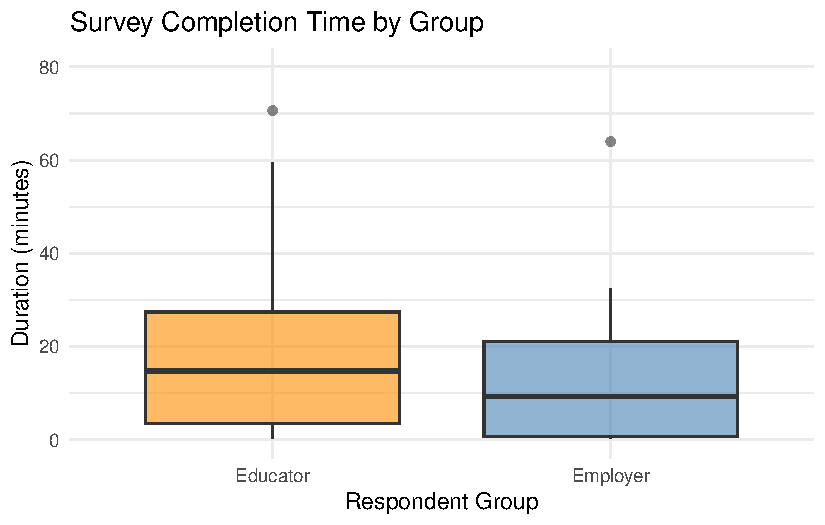
\includegraphics[keepaspectratio]{Final-Project_files/figure-pdf/Data_Desc_01-1.pdf}}

}

\caption{Assessing survey elapsed time distribution via box plots to
understand engagement by survey group.}

\end{figure}%

Survey completion time differed by group. Educators, on average, spent
more time completing the survey than employers. While no follow-up
question asked participants to explain their response time, this
discrepancy may reflect greater engagement or a tendency for more
elaborated responses among educators. It may also suggest a greater
willingness among educators to participate more thoughtfully. The box
plot below illustrates the distribution of survey duration (in minutes)
by group.

\begin{figure}[H]

{\centering \pandocbounded{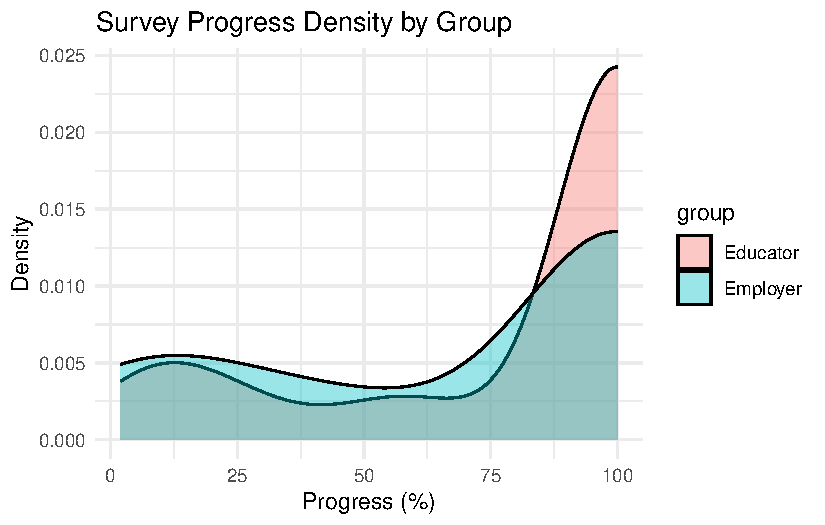
\includegraphics[keepaspectratio]{Final-Project_files/figure-pdf/Data_Desc_02-1.pdf}}

}

\caption{Assessing survey completion as a density curve to understand
engagement by survey group.}

\end{figure}%

Regarding the proportion of the survey completed, employer responses
were more variable---spanning the full range from partial to full
completion. In contrast, educators tended to complete more of the
survey, with a concentration near full completion and a less pronounced
left tail. The density plot below visualizes these differences in survey
progress across groups.

\begin{figure}[H]

{\centering \pandocbounded{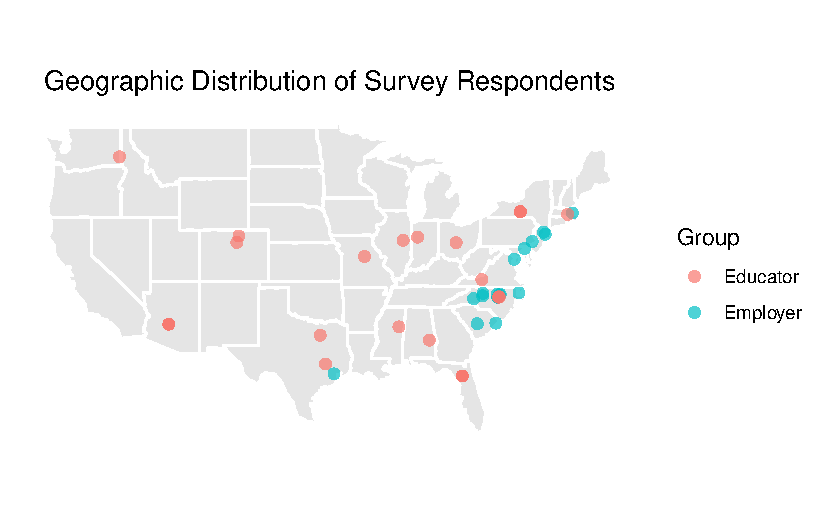
\includegraphics[keepaspectratio]{Final-Project_files/figure-pdf/Data_Desc_06-1.pdf}}

}

\caption{Geographic distribution of survey respondents across the United
States.}

\end{figure}%

Since our analysis focused on the representativeness of the United
States, we identified three sets of coordinates in the educator dataset
corresponding to international institutions: the University of Guelph in
Ontario, Canada; Zanzibar University in Chake, Tanzania; and Chiba
University in Chiba, Japan. Employer survey participants were
predominantly sampled from locations along the eastern seaboard of the
United States, while educators were more widely distributed across the
country. We highlight this to illustrate that perceptions of veterinary
dental students---particularly among employers---may differ for
individuals located far from the regions where most participants were
sampled. Additionally, because many of the responses came from major
metropolitan areas, our findings may underrepresent opinions regarding
student knowledge gaps in more rural settings.

\paragraph{Educator metrics}\label{educator-metrics}

\begin{figure}[H]

{\centering \pandocbounded{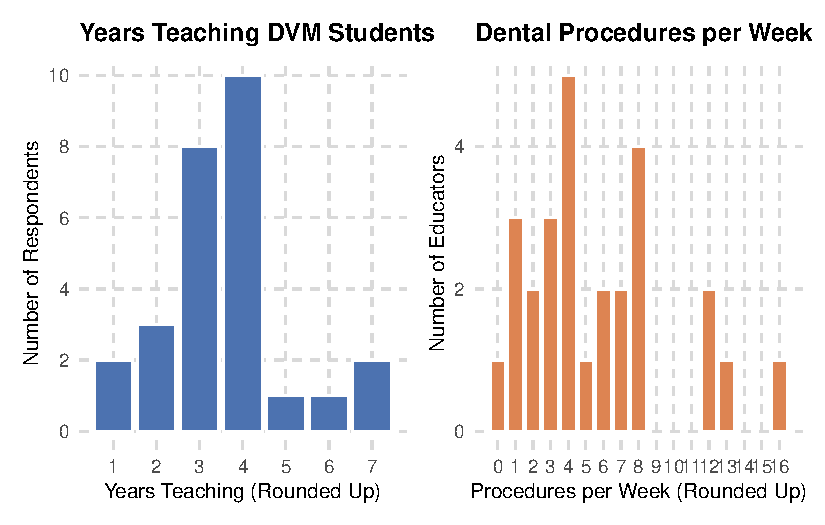
\includegraphics[keepaspectratio]{Final-Project_files/figure-pdf/Data_Desc_03-1.pdf}}

}

\caption{Educator contextualized background information about teaching
and procedures.}

\end{figure}%

Figure 3.3 provides an overview of the survey participants and their
institutions. Most respondents reported having between 2 and 4 years of
experience teaching veterinary students in clinical training. The
distribution of years taught appears approximately normal, with fewer
educators at the lower and upper ends of the experience range.
Respondents also reported the number of dental procedures performed by
their primary care service each week. While some outliers from busier
institutions reported higher volumes, most educators estimated
performing between 1 and 8 procedures per week.

\paragraph{Employer metrics}\label{employer-metrics}

\begin{longtable}[]{@{}lrr@{}}
\caption{Job Setting or Organization: Counts and
Percentages}\tabularnewline
\toprule\noalign{}
Job Setting & Count & Percentage \\
\midrule\noalign{}
\endfirsthead
\toprule\noalign{}
Job Setting & Count & Percentage \\
\midrule\noalign{}
\endhead
\bottomrule\noalign{}
\endlastfoot
Group corporate veterinary practice & 2 & 16.7 \\
Independently owned group veterinary practice & 2 & 16.7 \\
Independently owned single veterinary practice & 7 & 58.3 \\
Industry/commercial & 1 & 8.3 \\
\end{longtable}

\begin{longtable}[]{@{}lrr@{}}
\caption{Respondent Role: Counts and Percentages}\tabularnewline
\toprule\noalign{}
Respondent Role & Count & Percentage \\
\midrule\noalign{}
\endfirsthead
\toprule\noalign{}
Respondent Role & Count & Percentage \\
\midrule\noalign{}
\endhead
\bottomrule\noalign{}
\endlastfoot
Associate veterinarian & 2 & 18.2 \\
Practice manager/HR representative & 2 & 18.2 \\
Practice owner & 7 & 63.6 \\
\end{longtable}

Table 1 and Table 2 provide additional context about the survey
respondents. The majority of respondents work in privately owned
veterinary practices, and most identified themselves as the owners of
those practices.

\begin{figure}[H]

{\centering \pandocbounded{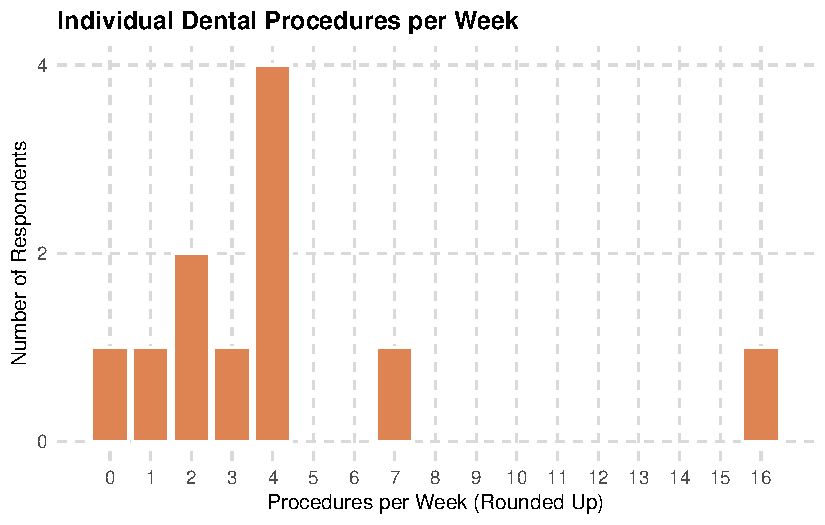
\includegraphics[keepaspectratio]{Final-Project_files/figure-pdf/Data_Desc_05-1.pdf}}

}

\caption{Average dental procedures employer survey participants
indicated they performed each week.}

\end{figure}%

Figure 3.5 shows that procedure counts tend to be lower in the employer
group compared to the educator group, although the overall distribution
shapes are similar. In both groups, the data exhibit a right-skewed
pattern, with most respondents reporting lower procedure counts and a
few outliers representing higher volumes. This pattern aligns with the
intuitive understanding that while some practices or institutions have
greater clinical demands on veterinarians, these cases are less
common---at least based on the survey responses.

\subsection{Data Source}\label{data-source}

Survey data were collected using Qualtrics, a cloud-based experience
management platform commonly used for gathering feedback and sentiment
across workforce domains. Participants from the educator survey were
recruited via email invitation sent by the researcher, using
pre-existing contact lists. Dr.~Ross-Estrada distributed the employer
survey to her personal and professional networks online. Participation
was voluntary and anonymous. There was no incentive offered for
completing the survey.

\subsection{Preprocessing Description}\label{preprocessing-description}

Although the employer and educator data sets shared a similar structure,
they were not identical. Most pre-processing steps were applied
uniformly across both data sets, with minor deviations where needed.

The data sets were imported into the RStudio environment (version
2024.04.1 Build 748). A new variable was created to label the data
source (``Educator'' or ``Employer'') for later grouping and
visualization. The existing respondent\_id column served as a unique
identifier and was treated as the primary key.

Initial cleaning involved removing extraneous metadata included by
Qualtrics---such as survey start and end times, IP addresses,
geolocation data, and question display logic---all of which were
irrelevant to the analysis. These columns were trimmed to streamline the
dataset for subsequent transformation and statistical work.

Column names in the original Qualtrics export were alphanumeric but
often ambiguous and misleading. Many variable names did not match the
corresponding survey question numbers. Our team manually mapped the
exported column names to their corresponding survey questions and
responses by referencing adjacent metadata fields and using deductive
reasoning. This process allowed us to build an index-based column naming
structure, which greatly improved the manageability and interpretability
of the dataset.

Before diving into question-specific analysis, we first identified the
subset of survey questions relevant to our research objectives. All
unrelated or out-of-scope items were removed. This step reduced the
employer dataset from 176 columns to 100, and the educator dataset from
171 columns to 102.

Several formatting inconsistencies also needed to be resolved. Some
multi-select questions appeared in the form of comma-separated text
responses within a single column, while others were exported into
multiple binary columns. Additionally, for certain questions, a response
option that received zero selections was dropped entirely by Qualtrics.
To standardize these issues, we implemented a script to ``explode''
comma-separated responses into individual binary columns. For dropped
columns, we manually reintroduced them as zero-filled dummy variables to
preserve the full response structure.

Finally, we filtered out participants who answered less than half of the
survey. We also excluded:

\begin{itemize}
\item
  Employers who responded ``No'' to the question: ``Do you work with
  early career veterinarians (someone who has graduated from a DVM
  program after May 2021)?''
\item
  Educators who responded ``No'' to: ``Do you teach in any capacity of
  the dental curriculum at your institution?''
\end{itemize}

After all preprocessing steps, the final cleaned datasets consisted of
13 employer participants and 30 educator participants.

\section{Statistical Methods}\label{statistical-methods}

\subsection{Method Description}\label{method-description}

\paragraph{Likert scale questions (statistical questions \#1,3, 6, and
8)}\label{likert-scale-questions-statistical-questions-13-6-and-8}

These questions use a Likert scale with response options: Strongly
Agree, Agree, Disagree, and Strongly Disagree across a variety of skills
and procedures. Given the ordinal nature of these responses, we will use
diverging stacked bar charts and summary tables to visually explore the
data, followed by a Mann-Whitney U Test for formal hypothesis testing.

The Mann-Whitney U Test is a non-parametric test used to assess whether
there is a statistically significant difference in the distributions of
ordinal or continuous variables between two independent groups. In this
case, educators and employers are assumed to be independent, consistent
with the survey design.

This test is appropriate for Likert-scale data because:

\begin{itemize}
\tightlist
\item
  It does not assume normality (unlike the t-test),
\item
  It respects the ordinal (ranked) structure of the data,
\item
  It retains statistical power in small samples.
\end{itemize}

\begin{longtable}[]{@{}lrrr@{}}
\caption{Mann-Whitney U Rank Summary Table}\tabularnewline
\toprule\noalign{}
Group & Sample.Size & Sum.of.Ranks & Mean.Rank \\
\midrule\noalign{}
\endfirsthead
\toprule\noalign{}
Group & Sample.Size & Sum.of.Ranks & Mean.Rank \\
\midrule\noalign{}
\endhead
\bottomrule\noalign{}
\endlastfoot
Group 1 (e.g., Educators) & n₁ & R₁ & R₁ / n₁ \\
Group 2 (e.g., Employers) & n₂ & R₂ & R₂ / n₂ \\
\end{longtable}

In order to calculate the test statistic and p-value for a Mann-Whitney
U Test:

\begin{itemize}
\tightlist
\item
  All observations are ranked together
\item
  The sum of the ranks for each group is calculated (\(R_1\) and
  \(R_2\))
\item
  The test statistic U is then calculated as the minimum of \(U_1\) and
  \(U_2\) where \(U_1\) and \(U_2\) are the following:
  \(U_1 = R_1 - \frac{n_1(n_1 + 1)}{2},  U_2 = R_2 - \frac{n_2(n_2 + 1)}{2}\)
\item
  Then the p-value is calculated from the U distribution or normal
  approximation.
\end{itemize}

P-values will be utilized for each statistical question listed above in
order to formally analyze the data.

\paragraph{Select all that apply questions (statistical questions \#2,
5, and
7)}\label{select-all-that-apply-questions-statistical-questions-2-5-and-7}

These questions asked the participants to ``select all that apply'' as
it relates to skills in pre-clinical curriculum, format of dental
instruction, and skills for clinical training respectively. We will
utilize frequency tables and bar plots to explore the data for these
questions and use Fisher's Exact Test as a formal inference procedure
for the comparison of the two groups. Dot plots will also be utilized
for questions with many options to avoid crowding in bar graphs.

Fisher's Exact Test works with categorical data with independent
samples, in this case educators and employers. Based on the survey
design from the client, it is again reasonable to assume that these two
groups are independent. In this context, Fisher's Exact Test is
preferred over Chi-Squared Tests due to the small sample size and
therefore not meeting the expected count threshold that is required to
proceed with Chi-Squared Tests. Given the small sample sizes, we
acknowledge the limited power of these analyses and may consider post
hoc power analyses for these tests.

\begin{longtable}[]{@{}
  >{\raggedright\arraybackslash}p{(\linewidth - 6\tabcolsep) * \real{0.3288}}
  >{\raggedleft\arraybackslash}p{(\linewidth - 6\tabcolsep) * \real{0.2192}}
  >{\raggedleft\arraybackslash}p{(\linewidth - 6\tabcolsep) * \real{0.2055}}
  >{\raggedright\arraybackslash}p{(\linewidth - 6\tabcolsep) * \real{0.2466}}@{}}
\caption{Fisher's Exact 2×2 Contingency Table}\tabularnewline
\toprule\noalign{}
\begin{minipage}[b]{\linewidth}\raggedright
Group
\end{minipage} & \begin{minipage}[b]{\linewidth}\raggedleft
Outcome.Present
\end{minipage} & \begin{minipage}[b]{\linewidth}\raggedleft
Outcome.Absent
\end{minipage} & \begin{minipage}[b]{\linewidth}\raggedright
Row.Totals
\end{minipage} \\
\midrule\noalign{}
\endfirsthead
\toprule\noalign{}
\begin{minipage}[b]{\linewidth}\raggedright
Group
\end{minipage} & \begin{minipage}[b]{\linewidth}\raggedleft
Outcome.Present
\end{minipage} & \begin{minipage}[b]{\linewidth}\raggedleft
Outcome.Absent
\end{minipage} & \begin{minipage}[b]{\linewidth}\raggedright
Row.Totals
\end{minipage} \\
\midrule\noalign{}
\endhead
\bottomrule\noalign{}
\endlastfoot
Group 1 (ex: Educators) & a & b & a + b \\
Group 2 (ex: Employers) & c & d & c + d \\
Column Totals & a + c & b + d & n = a + b + c + d \\
\end{longtable}

Fisher's Exact Test operates under the null hypothesis that there is no
association between the two variables. The alternative hypothesis is
that there is an association. The p-value for the test is computed using
the following formula:

\[p = \frac{(a+b)! \, (c+d)! \, (a+c)! \, (b+d)!}{a! \, b! \, c! \, d! \, n!}\]

P-values are then computed for each skill, format, etc. between the two
groups (educators and employers) depending on the statistical question
to be analyzed.

\paragraph{Numerical entry questions: (statistical question
\#4)}\label{numerical-entry-questions-statistical-question-4}

This question asks participants to enter a number related to the number
of dental procedures that should be completed during training in
different areas. We plan to produce box plots and/or histograms to
visually examine the data. Depending on the normality or lack thereof of
the distributions, we will then conduct either a two-sample t-test or a
Mann-Whitney U Test. As mentioned above, the Mann Whitney U test is a
non-parametric test that does not depend on the assumption of normality.
If the assumption on normality is met, we can consider a two-sample t
test for this analysis.

\section{Results}\label{results}

\subsection{Statistical Analysis}\label{statistical-analysis}

\subsubsection{S1 Are there significant differences between educators
and practice owners in their belief that new graduates are competent in
key dental skills on their first day of
practice?}\label{s1-are-there-significant-differences-between-educators-and-practice-owners-in-their-belief-that-new-graduates-are-competent-in-key-dental-skills-on-their-first-day-of-practice}

To assess whether there are differences in perceptions of new graduate
competence in dentistry, educators and employers were asked a parallel
question (Q4). Employers were asked to rate their expectation that early
career veterinarians can competently perform 12 specific dental skills
on their first day of employment. Educators were asked to rate whether
they believe new graduates can perform those same skills competently.
Responses were recorded on a 4-point Likert scale from 1 (Strongly
Disagree) to 4 (Strongly Agree).

We used the Mann-Whitney U test to compare the responses between
educators and employers for each skill. This non-parametric test is
appropriate for comparing ordinal data between two independent groups,
especially when the assumptions for parametric tests may not hold.
Ratings were reshaped into long format and analyzed skill-by-skill.
Median scores and group sizes were also reported to support
interpretation of the findings.

The results showed no statistically significant differences between
educators and employers for most skills, indicating general agreement
about which dental competencies new graduates possess. The only skill
approaching significance was interpreting dental radiographs (p =
0.064), where employers appeared slightly more confident than educators.
While this difference is subtle (both groups had a median rating of 3),
it may warrant further exploration in future studies. Overall, the
findings suggest alignment between educational preparation and employer
expectations regarding small animal dentistry skills.

\begin{table}
\caption*{
{\large Mann-Whitney U Test Results by Skill}
} 
\fontsize{12.0pt}{14.4pt}\selectfont
\begin{tabular*}{\linewidth}{@{\extracolsep{\fill}}lrrrrr}
\toprule
Skill & p-value & Median (Educator) & Median (Employer) & n (Educator) & n (Employer) \\ 
\midrule\addlinespace[2.5pt]
Q04\_03 & 0.064 & 3 & 3.0 & 30 & 12 \\ 
Q04\_10 & 0.242 & 2 & 3.0 & 30 & 13 \\ 
Q04\_05 & 0.260 & 3 & 3.0 & 30 & 13 \\ 
Q04\_06 & 0.396 & 3 & 3.0 & 30 & 13 \\ 
Q04\_02 & 0.485 & 3 & 2.5 & 29 & 12 \\ 
Q04\_04 & 0.492 & 4 & 4.0 & 29 & 13 \\ 
Q04\_09 & 0.533 & 2 & 2.0 & 29 & 13 \\ 
Q04\_08 & 0.728 & 3 & 3.0 & 30 & 13 \\ 
Q04\_01 & 0.872 & 4 & 4.0 & 30 & 13 \\ 
Q04\_07 & 0.955 & 3 & 3.0 & 30 & 13 \\ 
Q04\_11 & 1.000 & 1 & 1.0 & 8 & 4 \\ 
Q04\_12 & 1.000 & 3 & 4.0 & 2 & 1 \\ 
\bottomrule
\end{tabular*}
\end{table}

\subsubsection{S2 Is there a difference between educators and practice
owners in their reports (educators' actual teaching vs.~owners'
perceptions) of which dental skills were taught in the pre-clinical DVM
curriculum for recent
graduates?}\label{s2-is-there-a-difference-between-educators-and-practice-owners-in-their-reports-educators-actual-teaching-vs.-owners-perceptions-of-which-dental-skills-were-taught-in-the-pre-clinical-dvm-curriculum-for-recent-graduates}

To evaluate whether differences exist between DVM educators and
employers in their understanding of which dental skills are taught in
the pre-clinical curriculum, we analyzed responses to parallel survey
questions. Educators were asked to indicate which of seven core
dentistry skills are taught as part of their pre-clinical courses (Q12),
while employers were asked which skills they believe recent graduates
were taught prior to clinical training (Q16). Since the two groups
answered different question numbers about the same underlying skills, we
first aligned the datasets by renaming employer variables to match
educator labels. This harmonization allowed for direct comparison of
responses skill-by-skill across the two groups.

After cleaning and reshaping the data into long format, we filtered out
invalid or missing entries and conducted Fisher's Exact Tests for each
skill. This non-parametric test is appropriate for evaluating
categorical (yes/no) outcomes in small samples, especially when
comparing proportions between two independent groups. Only skills for
which both groups provided non-missing responses were included in the
final analysis. One skill item was excluded due to all responses being
missing, and approximately 70\% of employer data for Q16 items were
incomplete, limiting the strength of some comparisons.

The results of the Fisher's tests revealed no statistically significant
differences between educators and employers for any of the seven aligned
skills (all p-values \textgreater{} 0.32). Both groups reported similar
proportions of skills being taught, with educator endorsement rates
ranging from approximately 53\% to 77\%, and employer endorsement
ranging from 54\% to 92\%. These findings suggest general agreement
between what educators report teaching and what employers believe early
career veterinarians have been taught in the pre-clinical phase of
training. The overall consistency supports the idea that pre-clinical
dental training expectations are reasonably aligned between academic
programs and employer perceptions.

\begin{longtable}[]{@{}
  >{\raggedright\arraybackslash}p{(\linewidth - 10\tabcolsep) * \real{0.1831}}
  >{\raggedleft\arraybackslash}p{(\linewidth - 10\tabcolsep) * \real{0.1127}}
  >{\raggedleft\arraybackslash}p{(\linewidth - 10\tabcolsep) * \real{0.1549}}
  >{\raggedleft\arraybackslash}p{(\linewidth - 10\tabcolsep) * \real{0.1549}}
  >{\raggedleft\arraybackslash}p{(\linewidth - 10\tabcolsep) * \real{0.1972}}
  >{\raggedleft\arraybackslash}p{(\linewidth - 10\tabcolsep) * \real{0.1972}}@{}}
\caption{Fisher's Exact Test Results by Skill}\tabularnewline
\toprule\noalign{}
\begin{minipage}[b]{\linewidth}\raggedright
Skill\_Format
\end{minipage} & \begin{minipage}[b]{\linewidth}\raggedleft
p\_value
\end{minipage} & \begin{minipage}[b]{\linewidth}\raggedleft
n\_educator
\end{minipage} & \begin{minipage}[b]{\linewidth}\raggedleft
n\_employer
\end{minipage} & \begin{minipage}[b]{\linewidth}\raggedleft
prop\_educator
\end{minipage} & \begin{minipage}[b]{\linewidth}\raggedleft
prop\_employer
\end{minipage} \\
\midrule\noalign{}
\endfirsthead
\toprule\noalign{}
\begin{minipage}[b]{\linewidth}\raggedright
Skill\_Format
\end{minipage} & \begin{minipage}[b]{\linewidth}\raggedleft
p\_value
\end{minipage} & \begin{minipage}[b]{\linewidth}\raggedleft
n\_educator
\end{minipage} & \begin{minipage}[b]{\linewidth}\raggedleft
n\_employer
\end{minipage} & \begin{minipage}[b]{\linewidth}\raggedleft
prop\_educator
\end{minipage} & \begin{minipage}[b]{\linewidth}\raggedleft
prop\_employer
\end{minipage} \\
\midrule\noalign{}
\endhead
\bottomrule\noalign{}
\endlastfoot
Q12\_03 & 0.324 & 30 & 13 & 0.700 & 0.538 \\
Q12\_01 & 0.400 & 30 & 13 & 0.767 & 0.923 \\
Q12\_05 & 0.485 & 30 & 13 & 0.733 & 0.615 \\
Q12\_07 & 0.736 & 30 & 13 & 0.633 & 0.538 \\
Q12\_02 & 0.743 & 30 & 13 & 0.533 & 0.615 \\
Q12\_06 & 0.747 & 30 & 13 & 0.600 & 0.538 \\
Q12\_04 & 1.000 & 30 & 13 & 0.633 & 0.615 \\
\end{longtable}

\subsubsection{S3 Is there a difference between educators and practice
owners in their level of agreement about whether specific dental skills
should be taught
pre-clinically?}\label{s3-is-there-a-difference-between-educators-and-practice-owners-in-their-level-of-agreement-about-whether-specific-dental-skills-should-be-taught-pre-clinically}

To assess whether educators and employers differ in their beliefs about
which dental skills should be included in the pre-clinical DVM
curriculum, we analyzed responses to parallel Likert-scale questions:
Q13 (educators) and Q17 (employers). Both groups rated the importance of
teaching 12 specific dentistry skills using a 4-point Likert scale
ranging from 1 (Strongly Disagree) to 4 (Strongly Agree). Because the
data were ordinal and responses came from two independent groups, the
Mann-Whitney U test was used to compare educator and employer ratings
for each skill individually.

The results showed statistically significant differences in opinion for
two of the twelve skills. Employers were significantly more likely than
educators to agree that feline open extractions involving multiple roots
or canines (Skill\_11, p = 0.003) and fluoride treatment (Skill\_12, p =
0.013) should be included in the pre-clinical curriculum. For all other
skills, there were no statistically significant differences between
groups (all p \textgreater{} 0.10), and the median rating for most
skills was 4 (``Strongly Agree'') in both groups. These findings suggest
general alignment between educators and employers on most skills, but
highlight a few areas---particularly more advanced feline extractions
and fluoride use---where employer expectations may exceed what educators
currently prioritize for pre-clinical training.

\subsubsection{S4 Do employers and educators differ in their
expectations about how many dental procedures new graduates should
complete during clinical
training?}\label{s4-do-employers-and-educators-differ-in-their-expectations-about-how-many-dental-procedures-new-graduates-should-complete-during-clinical-training}

\subsubsection{S5 Is there difference between the instructional formats
in dentistry reported by DVM programs and the formats perceived by
employers to have been completed by early career
veterinarians?}\label{s5-is-there-difference-between-the-instructional-formats-in-dentistry-reported-by-dvm-programs-and-the-formats-perceived-by-employers-to-have-been-completed-by-early-career-veterinarians}

Both educators and employers were asked a question relating to the
format of instruction during the clinical year.

On question 20 of their survey, employers were asked: ``What format of
clinical instruction in dentistry do you believe that the early career
veterinarians (individuals who have graduated from a DVM program after
May 2021) hired into your practice/organization/institution completed as
part of their DVM training? Select all that apply.''

On question 16 of their survey, educators were asked: ``What format of
instruction in dentistry does your DVM program provide during the
clinical year? Select all that apply.''

Since the question was of the format ``select all that apply,''
participants were able to select more than one response and percentages
will not add to 100\%. Results reported below are the percentages of
their respective group (educators or employers) that selected the given
format of instruction. Percentages were utilized due to the difference
in sample size.

Educators and employers were also given the option to enter their own
responses to the question. One employer opted to write in ``Cadaver.''
Two educators entered their own responses with one saying ``rounds'' and
the other saying ``topic seminars do occur with some rotations during
case rounds when dental cases are chosen to present.''

Educators and employers differed in their perceptions of clinical dental
instruction formats completed by early career veterinarians. While a
majority in both groups acknowledged didactic instruction, educators
reported higher rates of wet lab (73.3\% vs.~46.2\%) and live patient
training (93.3\% vs.~38.5\%) compared to employers. Conversely,
employers more frequently identified simulation training (30.8\%
vs.~16.7\%) than educators. These differences suggest varying
expectations or awareness between the two groups regarding dental
training experiences of recent graduates.

\begin{figure}[H]

{\centering \pandocbounded{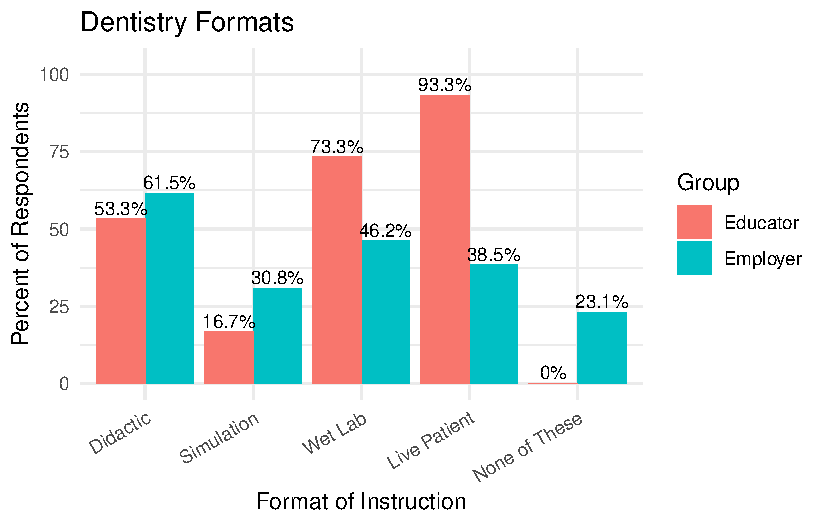
\includegraphics[keepaspectratio]{Final-Project_files/figure-pdf/formatgraph-1.pdf}}

}

\caption{Perceived Clinical Instruction Formats in Dentistry Completed
by Early Career Veterinarians}

\end{figure}%

Figure 5.1 shows the percentages of each format selected and Table 3
shows the p-value associated with performing Fisher's Exact Test on each
format.

Didactic instruction was selected by 53.3\% of educators and 61.5\% of
employers, with no statistically significant difference between the
groups (p=0.743). There was also no statistically significant difference
in simulation (p=0.417) and wet lab instruction (p=0.162).

On the other hand, live patient instruction was selected by 93.3\% of
educators, but only 38.5\% of employers. This difference was found to be
statistically significant with a p-value of 0.0003.

``None of these'' was also found to be statistically significant at the
5\% level. No educators selected that none of these formats were used,
but 23.1\% of employers selected that none of the formats were believed
to be utilized in the clinical year.

\begin{longtable}[]{@{}
  >{\raggedright\arraybackslash}p{(\linewidth - 6\tabcolsep) * \real{0.1867}}
  >{\raggedleft\arraybackslash}p{(\linewidth - 6\tabcolsep) * \real{0.3200}}
  >{\raggedleft\arraybackslash}p{(\linewidth - 6\tabcolsep) * \real{0.3200}}
  >{\raggedright\arraybackslash}p{(\linewidth - 6\tabcolsep) * \real{0.1733}}@{}}
\caption{Perceived Formats of Clinical Dental Instruction in DVM
Programs}\tabularnewline
\toprule\noalign{}
\begin{minipage}[b]{\linewidth}\raggedright
Format
\end{minipage} & \begin{minipage}[b]{\linewidth}\raggedleft
\% of Educators Selected
\end{minipage} & \begin{minipage}[b]{\linewidth}\raggedleft
\% of Employers Selected
\end{minipage} & \begin{minipage}[b]{\linewidth}\raggedright
P-value
\end{minipage} \\
\midrule\noalign{}
\endfirsthead
\toprule\noalign{}
\begin{minipage}[b]{\linewidth}\raggedright
Format
\end{minipage} & \begin{minipage}[b]{\linewidth}\raggedleft
\% of Educators Selected
\end{minipage} & \begin{minipage}[b]{\linewidth}\raggedleft
\% of Employers Selected
\end{minipage} & \begin{minipage}[b]{\linewidth}\raggedright
P-value
\end{minipage} \\
\midrule\noalign{}
\endhead
\bottomrule\noalign{}
\endlastfoot
Didactic & 53.3 & 61.5 & 0.743 \\
Simulation & 16.7 & 30.8 & 0.417 \\
Wet Lab & 73.3 & 46.2 & 0.162 \\
Live Patient & 93.3 & 38.5 & 0.000303 *** \\
None of These & 0.0 & 23.1 & 0.0232 * \\
\end{longtable}

\subsubsection{S6 Do educators and employers differ in their views on
which formats of clinical instruction in dentistry should be required
for DVM students as part of their clinical
training?}\label{s6-do-educators-and-employers-differ-in-their-views-on-which-formats-of-clinical-instruction-in-dentistry-should-be-required-for-dvm-students-as-part-of-their-clinical-training}

In question \#21 of the employers' version of the survey, participants
were asked:

\begin{itemize}
\tightlist
\item
  ``Which of the following types of \ul{clinical instruction} in
  dentistry do you think that DVM students should be required to
  complete as part of a \ul{DVM program}? Select one response for each
  of the instructional types listed below.''
\end{itemize}

The analogue of this question for educators was survey question \#17,
which asked:

\begin{itemize}
\tightlist
\item
  ``Which of the following types of \ul{instruction} do you think DVM
  students should be required to complete as part of their \ul{clinical
  training}? Select one response for each type of instruction listed
  below.''
\end{itemize}

This question aimed to assess how participants view the types of dental
instruction that should be required within veterinary medical curricula.
To examine whether there were differences in opinions between educators
and employers, the Mann-Whitney U-Test---a non-parametric test also
known as the Wilcoxon Rank-Sum Test---was used. This test is appropriate
for comparing two independent groups without assuming a normal
distribution and assumes mutual exclusivity between the groups.

\begin{longtable}[]{@{}
  >{\centering\arraybackslash}p{(\linewidth - 8\tabcolsep) * \real{0.2466}}
  >{\centering\arraybackslash}p{(\linewidth - 8\tabcolsep) * \real{0.1781}}
  >{\centering\arraybackslash}p{(\linewidth - 8\tabcolsep) * \real{0.1233}}
  >{\centering\arraybackslash}p{(\linewidth - 8\tabcolsep) * \real{0.1918}}
  >{\centering\arraybackslash}p{(\linewidth - 8\tabcolsep) * \real{0.2603}}@{}}
\caption{Mann-Whitney U-Test Results for Instruction
Types}\tabularnewline
\toprule\noalign{}
\begin{minipage}[b]{\linewidth}\centering
Instruction\_Type
\end{minipage} & \begin{minipage}[b]{\linewidth}\centering
W\_Statistic
\end{minipage} & \begin{minipage}[b]{\linewidth}\centering
P\_Value
\end{minipage} & \begin{minipage}[b]{\linewidth}\centering
Significance
\end{minipage} & \begin{minipage}[b]{\linewidth}\centering
Notes
\end{minipage} \\
\midrule\noalign{}
\endfirsthead
\toprule\noalign{}
\begin{minipage}[b]{\linewidth}\centering
Instruction\_Type
\end{minipage} & \begin{minipage}[b]{\linewidth}\centering
W\_Statistic
\end{minipage} & \begin{minipage}[b]{\linewidth}\centering
P\_Value
\end{minipage} & \begin{minipage}[b]{\linewidth}\centering
Significance
\end{minipage} & \begin{minipage}[b]{\linewidth}\centering
Notes
\end{minipage} \\
\midrule\noalign{}
\endhead
\bottomrule\noalign{}
\endlastfoot
Didactic & 138.5 & 0.415 & ns & Test performed \\
Simulation & 108 & 0.363 & ns & Test performed \\
Wet Lab & 162 & 0.713 & ns & Test performed \\
Live Patient & 263.5 & 0.003 & ** & Test performed \\
None of these & - & - & - & Insufficient data \\
Other & - & - & - & Insufficient data \\
\end{longtable}

The results are presented in Table 7. No statistically significant
differences were found between educators and employers in their
responses regarding the Didactic, Simulation, or Wet Lab instructional
formats. However, a significant difference was identified between the
two groups concerning Live Patient instruction, where responses varied
significantly. The instructional categories ``None of These'' and
``Other'' could not be tested due to insufficient data.

\subsubsection{S7 Is there a difference between the clinical dentistry
skills that educators report DVM students are learning during their
clinical training and the skills that employers believe recent graduates
have completed as part of their DVM
program?}\label{s7-is-there-a-difference-between-the-clinical-dentistry-skills-that-educators-report-dvm-students-are-learning-during-their-clinical-training-and-the-skills-that-employers-believe-recent-graduates-have-completed-as-part-of-their-dvm-program}

Both educators and employers were asked a question related to skills
learned and practiced during the clinical year.

On question 25 of their survey, employers were asked: ``Which of the
following skills do you think that individuals who graduated with a DVM
degree after May 2021 completed during the clinical training portion of
their DVM program? Select all that apply.''

On question 20 of their survey, educators were asked: ``Which of the
following skills are DVM students at your institution
practicing/learning during the clinical training portion of the DVM
program? Select all that apply.''

Since the question was of the format ``select all that apply,''
participants were able to select more than one response and percentages
will not add to 100\%. Results reported below are the percentages of
their respective group (educators or employers) that selected the given
format of instruction. Percentages were utilized due to the difference
in sample size.

Educators and employers were also given the option to enter their own
responses to the question. No employers entered any text responses. Six
educators entered text responses of the following:

\begin{itemize}
\tightlist
\item
  ``OvaVet gel application, Crown amputation, Sealant application for
  UCF, oral tumor biopsy and excision, orthodontia''
\item
  ``Nerve blocks, barrier sealant and bonded sealant application, jaw
  fracture repair, root canals''
\item
  ``Often- bonded sealants; Sometimes- root canals, restorations, jaw
  fracture repair''
\item
  ``Oral biopsy, root planning, bonded sealants''
\item
  ``extractions only if performed on that patient''
\item
  ``Not all students see all types of extractions''
\end{itemize}

\begin{figure}[H]

{\centering \pandocbounded{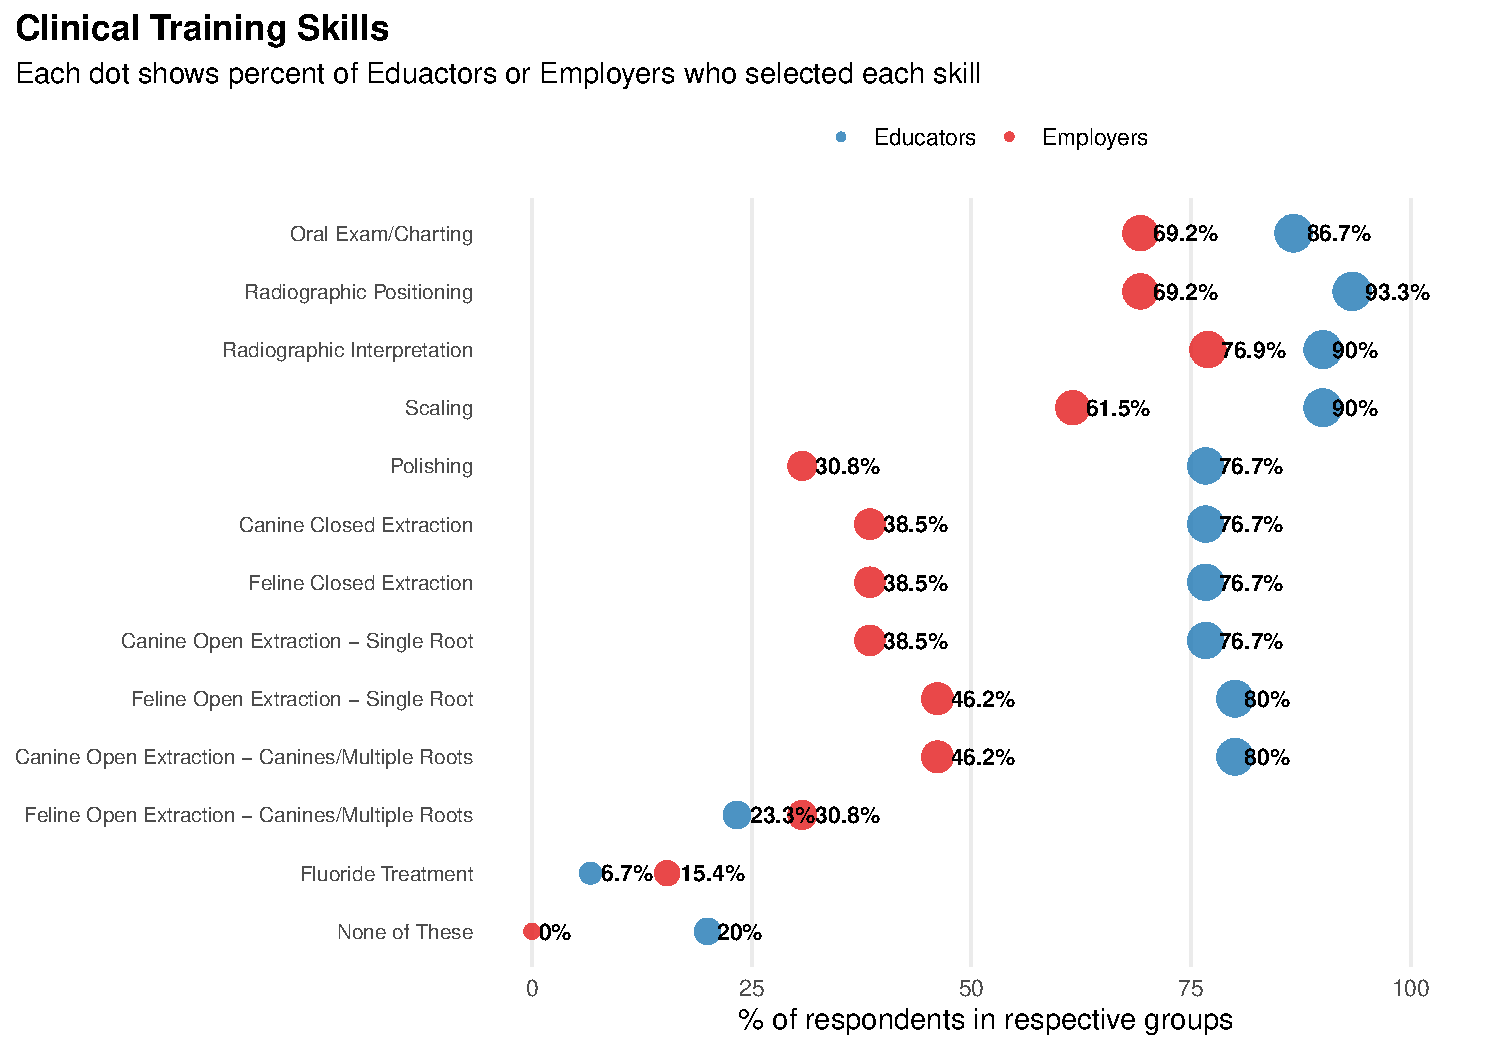
\includegraphics[keepaspectratio]{Final-Project_files/figure-pdf/question_7a-1.pdf}}

}

\caption{Clinical Training Skills Perceived by Educators vs Employers in
DVM Programs}

\end{figure}%

\begin{longtable}[]{@{}
  >{\raggedright\arraybackslash}p{(\linewidth - 6\tabcolsep) * \real{0.5393}}
  >{\raggedleft\arraybackslash}p{(\linewidth - 6\tabcolsep) * \real{0.1685}}
  >{\raggedleft\arraybackslash}p{(\linewidth - 6\tabcolsep) * \real{0.1685}}
  >{\raggedright\arraybackslash}p{(\linewidth - 6\tabcolsep) * \real{0.1236}}@{}}
\caption{Perceived Skills Learned of Clinical Dental Instruction in DVM
Programs}\tabularnewline
\toprule\noalign{}
\begin{minipage}[b]{\linewidth}\raggedright
Skill
\end{minipage} & \begin{minipage}[b]{\linewidth}\raggedleft
\% of Educators
\end{minipage} & \begin{minipage}[b]{\linewidth}\raggedleft
\% of Employers
\end{minipage} & \begin{minipage}[b]{\linewidth}\raggedright
P-value
\end{minipage} \\
\midrule\noalign{}
\endfirsthead
\toprule\noalign{}
\begin{minipage}[b]{\linewidth}\raggedright
Skill
\end{minipage} & \begin{minipage}[b]{\linewidth}\raggedleft
\% of Educators
\end{minipage} & \begin{minipage}[b]{\linewidth}\raggedleft
\% of Employers
\end{minipage} & \begin{minipage}[b]{\linewidth}\raggedright
P-value
\end{minipage} \\
\midrule\noalign{}
\endhead
\bottomrule\noalign{}
\endlastfoot
Oral Exam/Charting & 86.7 & 69.2 & 0.217 \\
Radiographic Positioning & 93.3 & 69.2 & 0.0576 \\
Radiographic Interpretation & 90.0 & 76.9 & 0.345 \\
Scaling & 90.0 & 61.5 & 0.0415 * \\
Polishing & 76.7 & 30.8 & 0.00672 ** \\
Canine Closed Extraction & 76.7 & 38.5 & 0.0339 * \\
Feline Closed Extraction & 76.7 & 38.5 & 0.0339 * \\
Canine Open Extraction - Single Root & 76.7 & 38.5 & 0.0339 * \\
Feline Open Extraction - Single Root & 80.0 & 46.2 & 0.0367 * \\
Canine Open Extraction - Canines/Multiple Roots & 80.0 & 46.2 & 0.0367
* \\
Feline Open Extraction - Canines/Multiple Roots & 23.3 & 30.8 & 0.709 \\
Fluoride Treatment & 6.7 & 15.4 & 0.572 \\
None of These & 20.0 & 0.0 & 0.155 \\
\end{longtable}

Figure 5.2 shows the percentage of employers and educators who selected
the given skills and Table 4 shows the p-values associated with Fisher's
Exact Test and their significance.

For eleven of the thirteen skills, educators reported a higher
percentage of selection. The two skills for which employers reported
higher perceived learning were feline open extraction - canines/multiple
roots and fluoride treatment.

At the 5\% significance level, the difference in skill selection between
employers and educators was found to be significant for seven skills:

\begin{itemize}
\tightlist
\item
  Scaling
\item
  Polishing
\item
  Canine Closed Extraction
\item
  Feline Closed Extraction
\item
  Canine Open Extraction - Single Root
\item
  Feline Open Extraction - Single Root
\item
  Canine Open Extraction - Canines/Multiple Roots
\end{itemize}

For all skills with statistically significant differences, educators
reported higher percentages than employers.

The most significant difference was found in polishing. Educators
selected this skill 76.7\% of the time, while employers selected this
skill only 30.8\% of the time. The resulting p-value was 0.00672.

\subsubsection{S8 Do educators and employers differ in their opinions
about which clinical dentistry skills DVM students should be required to
practice or learn during their clinical
training?}\label{s8-do-educators-and-employers-differ-in-their-opinions-about-which-clinical-dentistry-skills-dvm-students-should-be-required-to-practice-or-learn-during-their-clinical-training}

In question \#26 of the employers' version of the survey, participants
were asked:

\begin{itemize}
\tightlist
\item
  ``Which of the following skills do you think that DVM students should
  be required to practice/learn as part of the clinical training portion
  of a DVM program? Select one response for each of the skills listed
  below.''
\end{itemize}

The corresponding question for educators was survey question \#21.

This question aimed to assess opinions on which clinical dentistry
skills should be required in DVM student training. To evaluate whether
differences existed between educators and employers, the Mann-Whitney
U-Test, a non-parametric test also known as the Wilcoxon Rank-Sum Test,
was applied. This test compares two independent groups without assuming
normality and requires mutual exclusivity between groups.

The results are presented in Table 9. No statistically significant
differences were observed between educators and employers for most of
the listed clinical skills, including oral examination/charting,
radiographic positioning, radiographic interpretation, scaling,
polishing, or several extraction procedures. However, significant
differences were identified for the skills of feline closed extraction
and canine open extraction---single root, with p-values of 0.049 for
both. Two additional procedures---feline open extraction---single root
and canine open extraction---canines/multiple roots---approached
significance (p = 0.076). The ``Fluoride treatment'' and ``None''
categories could not be tested due to insufficient data.

\begin{longtable}[]{@{}
  >{\centering\arraybackslash}p{(\linewidth - 8\tabcolsep) * \real{0.4712}}
  >{\centering\arraybackslash}p{(\linewidth - 8\tabcolsep) * \real{0.1250}}
  >{\centering\arraybackslash}p{(\linewidth - 8\tabcolsep) * \real{0.0865}}
  >{\centering\arraybackslash}p{(\linewidth - 8\tabcolsep) * \real{0.1346}}
  >{\centering\arraybackslash}p{(\linewidth - 8\tabcolsep) * \real{0.1827}}@{}}
\caption{Mann-Whitney U-Test Results for Clinical
Procedures}\tabularnewline
\toprule\noalign{}
\begin{minipage}[b]{\linewidth}\centering
Instruction\_Type
\end{minipage} & \begin{minipage}[b]{\linewidth}\centering
W\_Statistic
\end{minipage} & \begin{minipage}[b]{\linewidth}\centering
P\_Value
\end{minipage} & \begin{minipage}[b]{\linewidth}\centering
Significance
\end{minipage} & \begin{minipage}[b]{\linewidth}\centering
Notes
\end{minipage} \\
\midrule\noalign{}
\endfirsthead
\toprule\noalign{}
\begin{minipage}[b]{\linewidth}\centering
Instruction\_Type
\end{minipage} & \begin{minipage}[b]{\linewidth}\centering
W\_Statistic
\end{minipage} & \begin{minipage}[b]{\linewidth}\centering
P\_Value
\end{minipage} & \begin{minipage}[b]{\linewidth}\centering
Significance
\end{minipage} & \begin{minipage}[b]{\linewidth}\centering
Notes
\end{minipage} \\
\midrule\noalign{}
\endhead
\bottomrule\noalign{}
\endlastfoot
Oral exam/charting & 139 & 0.622 & ns & Test performed \\
Radiographic positioning & 157 & 0.717 & ns & Test performed \\
Radiographic interpretation & 126.5 & 0.194 & ns & Test performed \\
Scaling & 156 & 0.762 & ns & Test performed \\
Polishing & 148.5 & 1 & ns & Test performed \\
Canine closed extraction & 127.5 & 0.328 & ns & Test performed \\
Feline closed extraction & 104.5 & 0.049 & * & Test performed \\
Canine open extraction - Single root & 104.5 & 0.049 & * & Test
performed \\
Feline open extraction - Single root & 115.5 & 0.076 & . & Test
performed \\
Canine open extraction - Canines/multiple roots & 115.5 & 0.076 & . &
Test performed \\
Feline open extraction - Canines/multiple roots & 54 & 0.207 & ns & Test
performed \\
Fluoride treatment & - & - & - & Insufficient data \\
None & - & - & - & Insufficient data \\
\end{longtable}

\section{Discussion/Conclusion}\label{discussionconclusion}

\subsection{Interpretation of Results}\label{interpretation-of-results}

\subsection{Implications of the Study}\label{implications-of-the-study}

\subsection{Limitations}\label{limitations}

\subsection{Recommendations}\label{recommendations}

\subsection{Summary of Key Findings}\label{summary-of-key-findings}

\subsection{Final Thoughts}\label{final-thoughts}

\section{Appendix}\label{appendix}




\end{document}
